\begin{center}
\scriptsize
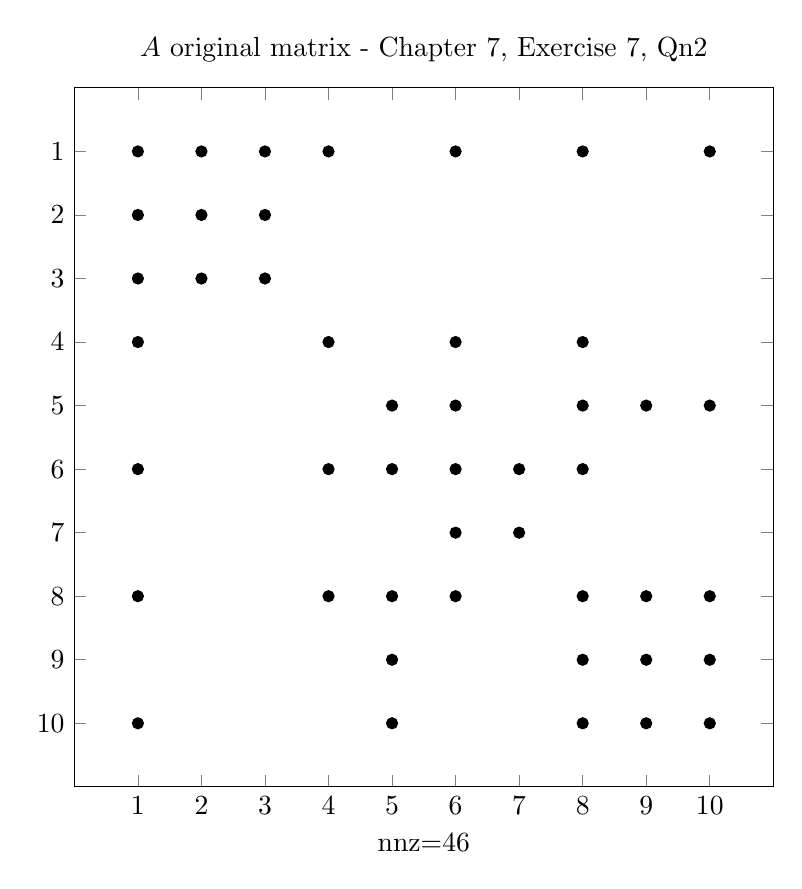
\begin{tikzpicture}
    [   baseline = {(current bounding box.north)}
    ]
    \begin{axis}
        [   unit vector ratio* = 1 1 1
        ,   y dir = reverse
        ,   xmin = 0
        ,   ymin = 0
        ,   xmax = 11
        ,   ymax = 11
        ,   title = {$A$ original matrix - Chapter 7, Exercise 7, Qn2}
        ,   xlabel = {nnz=46}
        ,   width = \linewidth
        ,   xtick = {1,2,3,4,5,6,7,8,9,10}
        ,   ytick = {1,2,3,4,5,6,7,8,9,10}
        ]
        \addplot[only marks] coordinates
        {   (1,1)(2,1)(3,1)(4,1)     (6,1)     (8,1)     (10,1)
            (1,2)(2,2)(3,2)
            (1,3)(2,3)(3,3)
            (1,4)          (4,4)     (6,4)     (8,4)
                                (5,5)(6,5)     (8,5)(9,5)(10,5)
            (1,6)          (4,6)(5,6)(6,6)(7,6)(8,6)
                                     (6,7)(7,7)
            (1,8)          (4,8)(5,8)(6,8)     (8,8)(9,8)(10,8)
                                (5,9)          (8,9)(9,9)(10,9)
            (1,10)              (5,10)      (8,10)(9,10)(10,10)
        };
    \end{axis}
\end{tikzpicture}
\end{center}
